\chapter{Containers}
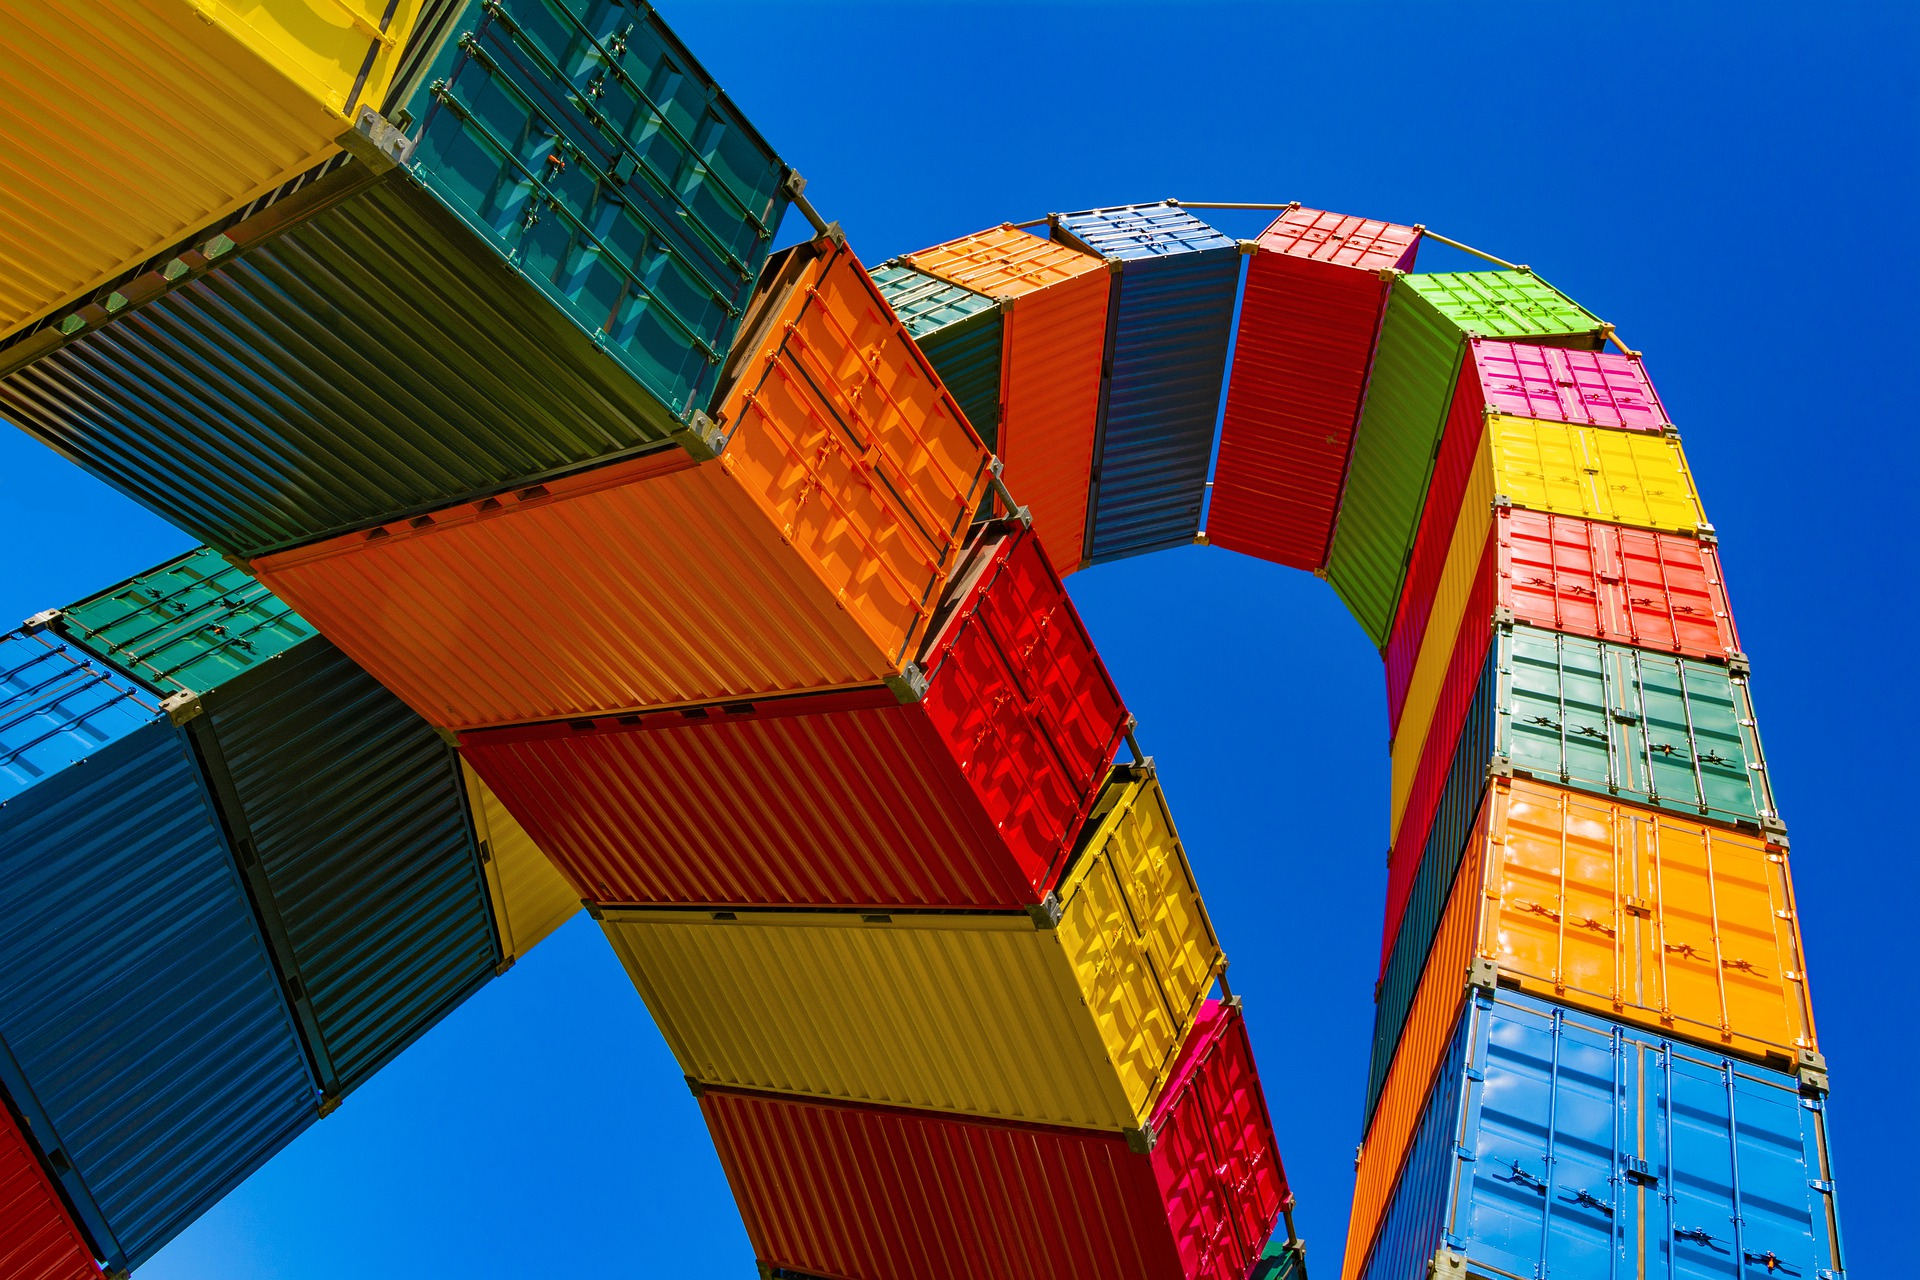
\includegraphics[scale=0.85]{../images/container-4203677_1920.jpg}
\justify
Containerization is the process of encapsulating the
code and dependencies for part or all of a project. 
The most popular and common tool for realizing
containerization is Docker\index{Docker}. Using Docker,
we can programatically build an environment for our project,
and pass the entirety of this encapsulated environment
from our local development machine, into the
Continuous Integration (CI)\index{Continuous Integraion}
pipeline for testing, and eventually into our production
environment. Containerization\index{containerization}
helps us by offering a consistent operating experience
across disparate environments.
\justify
Recall our earlier discussion on the topics of immutability\index{immutability}
and ephemerality\index{ephemerality}. 
It is more desirable to create projects that are built
and replaced frequently, than it is to attempt to upgrade
and repair the infrastructure, platforms, and project code
on an on-going basis. The reason this is more desirable 
is that attempts to patch and upgrade project
hosts "in place", quickly reveal great difficulty in maintaining consistency
with the project source. This is our only option when it comes 
to "bare metal" hosts, and some confgurations of hosts using
certain virtualization technologies. A lesser degree of immutability
and ephemerality also introduces issues keeping
operating system packages current, yet still compatible with
the project. Imagine a situation where an upgrade to a package
is necessary to meet security requirements, but this very same
upgrade means the project will stop working since the package
features that your application depends on have also changed.
The result is most likely angry end users and customers. 
Certainly not a situation we ever like to find ourselves in.

\justify
Docker images are "canned" (as in, prefabricated) or custom directives
for provisioning the operating system of a Docker container. One or more
images can be used as building blocks when configuring our containers.
For example, a base Linux image and base Python image might be combined
with our customizations that describe and point to our application code,
all of which make up a single container that provides the functions of
a fully provisioned server. We get the added
benefit of being able to switch quickly between base operating system
images with just a few lines of code change to our project. For example,
we could easily modify our container image to be predicated on Debian
rather than Red Hat distribution of Linux kernel and operating system
should the need arise.

\justify
See the Docker website for instructions on how to install and configure
Docker. A properly
functioning Docker setup on your local machine is a requirement for the
exercises we will do later. Note that Podman is an acceptable substitute
for Docker, as detailed later in this chapter.

\justify
Once you have Docker installed and running on your workstation, take a
look at the two example files below. For now it's OK to see them and get
a general familiarity with their contents. Later we will use these files
to create containers for our projects.

\section{Dockerfile}
\justify
The Dockerfile is our basic unit of containerization. That is to say,
our containers, and the applications they contain, are defined by the
Dockerfile. This Dockerfile will dictate how we provision resources and
include operating system essentials and packages inside our container.
Each Dockerfile is predicated on a base image, such as Python/Debian 10
as shown in the example below.

\justify
Consider a directory named
\href{https://github.com/hotpeppersec/rapid_secdev_framework/tree/master/docker}{Docker}
and a file called
\href{https://github.com/hotpeppersec/rapid_secdev_framework/blob/master/docker/Dockerfile}{Dockerfile}\index{Dockerfile}
within this directory. Note the capitalization of the first letter in the file name. Some IDE's will key off this file and allow for additional syntax highlighting.

\justify
\begin{mybox}{\thetcbcounter: Dockerfile}
  \lstinputlisting{code/04_docker/Dockerfile}
\end{mybox}

\justify
A valid Dockerfile begins with the \textbf{FROM} instruction. This
instruction specifies the base image that we will use to build our
project on. These base images come from the
\href{https://docs.docker.com/docker-hub/repos/}{Docker Hub
  repositories}. We are setting an environment variable
\textbf{DEBIAN\_FRONEND} to the value of noninteractive, which will
cause the apt command to skip or ignore any interactive menus that are
encountered during execution of the apt command, since these would cause
our builds to "hang up" at an inaccessible interactive prompt. The
\textbf{ADD} and \textbf{WORKDIR} directives are meant to cause Docker
to use the /workdir directory as the root of the project "inside" the
container. Finally, we are directing Docker to \textbf{RUN} and apt
update and install the apt-utils package.

\subsection{docker-compose.yml}
\justify
The docker-compose tool and its associated docker-compose.yml file
allows us to manage multiple Docker containers for one or more
applications. We will add this file to our project to illustrate it's
composition and give ourselves the ability to extend our work later, as
needed.

\justify
A file called docker-compose.yml\index{docker-compose.yml} will exist alongside our Dockerfile in our docker directory.

\begin{mybox}{\thetcbcounter: Example docker-compose.yml}
  version: '3'\\
  services:\\
  \hspace*{7mm}devsecops:\\
  \hspace*{15mm}hostname: devsecops\\
  \hspace*{15mm}container\_name: devsecops\\
  \hspace*{7mm}volumes:\\
  \hspace*{15mm}- ..:/project\\
  \hspace*{7mm}build:\\
  \hspace*{15mm}context: ..\\
  \hspace*{15mm}dockerfile: docker/Dockerfile
\end{mybox}

\justify
The docker-compose.yml file begins with a version specification. It's
important to note that the commands and structure of docker-compose.yml
can vary widely based on this version. While versions cannot be mixed,
all version are valid with respect to docker-compose itself. Wew specify
a service named "devsecops", and assign a host and container name. Under
"volumes" we are mounting the base of the project directory in the host
filesystem as "/project" in the container filesystem. The build
"directive" tells docker-compose how to locate the Dockerfile we wish to
use for the containers.

\subsection{Exercise: Testing Out Docker}
\justify
With Docker properly installed and an understanding of the necessary
configuration files, we can now try out our configuration. See
({myFig1}) for an illustration of how to lay out the project files in your local filesystem.


\begin{figure}[!htb]
  \centering
  
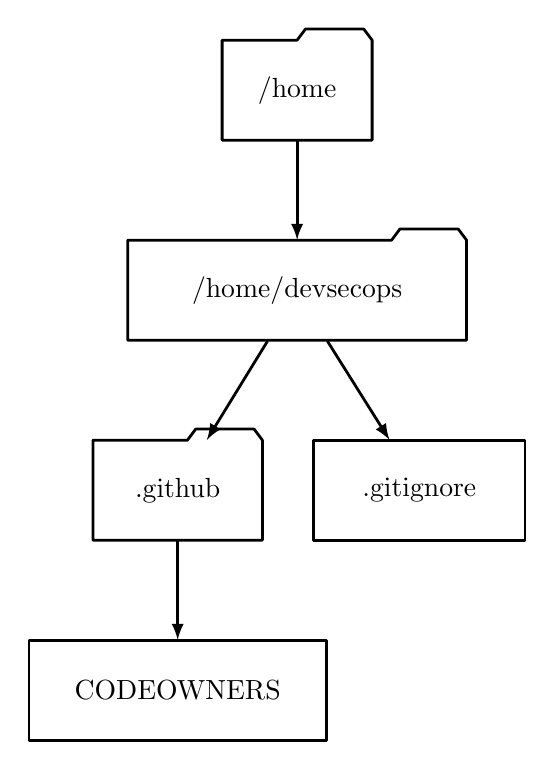
\begin{tikzpicture}[>=latex,line join=bevel,]
  \pgfsetlinewidth{1bp}
%%
\pgfsetcolor{black}
  % Edge: home -> devsecops
  \draw [->] (96.5bp,215.7bp) .. controls (96.5bp,207.98bp) and (96.5bp,198.71bp)  .. (96.5bp,180.1bp);
  % Edge: devsecops -> github
  \draw [->] (85.871bp,143.7bp) .. controls (80.872bp,135.56bp) and (74.809bp,125.69bp)  .. (64.007bp,108.1bp);
  % Edge: devsecops -> gitignore
  \draw [->] (107.38bp,143.7bp) .. controls (112.49bp,135.56bp) and (118.7bp,125.69bp)  .. (129.75bp,108.1bp);
  % Edge: github -> codeowners
  \draw [->] (53.5bp,71.697bp) .. controls (53.5bp,63.983bp) and (53.5bp,54.712bp)  .. (53.5bp,36.104bp);
  % Node: home
\begin{scope}
  \definecolor{strokecol}{rgb}{0.0,0.0,0.0};
  \pgfsetstrokecolor{strokecol}
  \draw (123.5bp,252.0bp) -- (120.5bp,256.0bp) -- (99.5bp,256.0bp) -- (96.5bp,252.0bp) -- (69.5bp,252.0bp) -- (69.5bp,216.0bp) -- (123.5bp,216.0bp) -- cycle;
  \draw (96.5bp,234.0bp) node {/home};
\end{scope}
  % Node: devsecops
\begin{scope}
  \definecolor{strokecol}{rgb}{0.0,0.0,0.0};
  \pgfsetstrokecolor{strokecol}
  \draw (157.5bp,180.0bp) -- (154.5bp,184.0bp) -- (133.5bp,184.0bp) -- (130.5bp,180.0bp) -- (35.5bp,180.0bp) -- (35.5bp,144.0bp) -- (157.5bp,144.0bp) -- cycle;
  \draw (96.5bp,162.0bp) node {/home/devsecops};
\end{scope}
  % Node: github
\begin{scope}
  \definecolor{strokecol}{rgb}{0.0,0.0,0.0};
  \pgfsetstrokecolor{strokecol}
  \draw (84.0bp,108.0bp) -- (81.0bp,112.0bp) -- (60.0bp,112.0bp) -- (57.0bp,108.0bp) -- (23.0bp,108.0bp) -- (23.0bp,72.0bp) -- (84.0bp,72.0bp) -- cycle;
  \draw (53.5bp,90.0bp) node {.github};
\end{scope}
  % Node: gitignore
\begin{scope}
  \definecolor{strokecol}{rgb}{0.0,0.0,0.0};
  \pgfsetstrokecolor{strokecol}
  \draw (178.5bp,108.0bp) -- (102.5bp,108.0bp) -- (102.5bp,72.0bp) -- (178.5bp,72.0bp) -- cycle;
  \draw (140.5bp,90.0bp) node {.gitignore};
\end{scope}
  % Node: codeowners
\begin{scope}
  \definecolor{strokecol}{rgb}{0.0,0.0,0.0};
  \pgfsetstrokecolor{strokecol}
  \draw (107.0bp,36.0bp) -- (0.0bp,36.0bp) -- (0.0bp,0.0bp) -- (107.0bp,0.0bp) -- cycle;
  \draw (53.5bp,18.0bp) node {CODEOWNERS};
\end{scope}
%
\end{tikzpicture}


  \caption{Project Directory and Docker related files.}
\end{figure}

\clearpage
\justify
Here is a step by step description of how to prepare the creation of our first container:

\begin{itemize}
  \item Create the "rapid\_secdev\_framework" folder.
        \begin{itemize}
          \item When creating folders, note that capitalization matters.
        \end{itemize}
  \item In that folder, create another folder called "docker".
  \item Now in the docker folder, create a text file with the name "Dockerfile".
        \begin{itemize}
          \item
                Copy and paste the example Dockerfile from earlier in this chapter
                into your text file.
        \end{itemize}
  \item Also in the docker folder, create a text file with the name "docker-compose.yml"
        \begin{itemize}
          \item Copy and paste the example docker-compose.yml file from earlier in this chapter into your second text file.
        \end{itemize}
\end{itemize}

\justify
Here is an example of the BASH shell commands you can use to accomplish
the steps of the exercise. You can substitue vi for your favorite text
editor as needed. Note that typing the "docker-compose" command on line
6 will reference the devsecops "service" we specified on line 3 of the
docker-compose.yml file.

\justify
\begin{mybox}{\thetcbcounter: Create files for Docker,height=3.5cm}
  mkdir rapid\_secdev\_framework\\
  cd rapid\_secdev\_framework\\
  mkdir docker\\
  vi docker/Dockerfile\\
  vi docker/docker-compose.yml
\end{mybox}

\justify
With our files created and populated, we are ready to generate our
container based on our specified configuration.

\begin{mybox}{\thetcbcounter: Build from docker-compose.yml }
  docker-compose -f docker/docker-compose.yml build devsecops
\end{mybox}

\justify
If all went well, you should now have a shell prompt from "inside" the
new container. Recall that we set our \textbf{WORKDIR} variable to /project in the Dockerfile. Following that example, we now have Dockerfile and docker-compose.yml in the directory /project/docker, having mounted the project directory from the host machine "inside" the container.

\subsubsection{Testing from GitHub}
\justify
In the next chapter
we will explore how to "clone" a project repository from 
\href{github.com} and
do our work directory from there.

\section{Security Scanning Our Containers}
The \href{trivy container scanner}{https://github.com/aquasecurity/trivy} bills itself as "A Simple and
Comprehensive Vulnerability Scanner for Containers and other
Artifacts, Suitable for CI".

\section{Substituting Podman for Docker}
\justify
Podman is an Open Source tool from the Open
Containers Initiative (OCI)\index{Open Containers Initiative
(OCI)}. The Podman\index{Podman} service is said to be capable
of being a drop-in replacement for Docker, although it only
runs on Linux hosts at the time of this writing. Podman gives
the user the ability to use traditional Docker commands,
without the need to run a daemon to do so\cite{podman}, as is
the case with Docker.

\justify
You can install Podman by 
\href{https://podman.io/getting-started/installation.html}{following the instructions}
at their web site. Once Podman is installed properly you
should be able to alias docker=podman and use it as a
drop-in replacement for Docker and it's associated daemon.

\section{Container Orchestration}
\justify
An orchestrator for containers can be thought of as an engine which
allows for their provisioning, deployment, scaling, monitoring, load
balancing, and more. The Container Orchestrator manages the
lifecycle and visibility of a container at all stages.

\justify
Kubernetes\index{Kubernetes} is an example, perhaps even the
penultimate example, of a Container Orchestrator\index{orchestration}.
Folks throughout the DevSecOps, Software and
Security communities are using Kubernetes these days, and
with good reason. It's adoption as a means to manage and
replicate containers, and scale the applications they contain,
has been nothing short of revolutionary. System administrators
and developers can do more, better work. Granted, this comes at
the expense of introduction yet another framework to learn, and
no small amount of complexity.

\justify
An orchestrator helps us achieve immutability, and scale
to meet user demand quickly and easily by abstracting away
concerns that come with operating workloads in a bare metal
or VM environment.

\justify
Kubernetes and other orchestrators are rapidly evolving. To ignore this
game-changing ecosystem is to be left behind in terms of technological
prowess. Learning about containers, pipelines, infrastructure, and
so on are the foundational elements you will want to become familiar
with in preparation for expanding your mindset into the greater
dimensionality that orchestration realizes.

\justify
Later we will look more closely at the sprawling and vibrant 
topic of Kubernetes. For this stage of our journey to DevSecOps
enlightenment, it is enough to know that orchestration exists
and have a bit of familiarity with its purpose.

\section{Further Reading}
